\chapter{Introduction}
\label{sec:intro}


This thesis is focused on robust motion planning for a nonlinear system model.
Planning with uncertainty is necessary in order for an algorithm to move out of
the lab and into the real world as in reality there are always uncertainty in
planning. Knowledge of position, the environment and the dynamics of the system
are all uncertain to some degree. Sensory noise, tuning and readings may be off.
Limited precision, and accidents may hinder the measurements and leave them with
an error term. Thus in order for a planner to guarantee safe traversal through a
real world environment, a motion planner needs to handle uncertainties. Over the
last couple of decades a lot of research has gone in to handling uncertianty in
planning, an overview of which can be found in \cref{chp:survey-of-papers}.


The \rrtfunnel{} algorithm is the answer provided to handle a subset of these
problems. As it currently stands the algorithm handles uncertainty only in the
position of the dynamical system, but can be easily extended to handle
uncertainty in input and speed as well. Handling uncertainties in the
environment is currently not handled.


The algorithm is built up through two main parts. One is the calculation of
\textit{robust motion primitives}, which allows the global motion planner (in
essence a regular \ac{RRT} algorithm) to remain completely oblivious to these
difficulties, and hence act as though there were no uncertainties during the
planning stage. This means that a lot of the difficulty of planning is handled
during the off-line phase of generating the robust motion primitives themselves.
This is done through the theory of \ac{SOS} programming and verification.
Through formulating the search for a \textit{Lyapunov function} for the system
as a \ac{SOS} program, the trajectories are extended to so called `funnels',
which incorporate all the states the system can be in during a given time frame
-- even in the face of uncertainties. In the literature this is referred to as a
\textit{finite time reachable set}, meaning that if the calculations are
correct, it contains all the states that the system can evolve to given a set of
initial conditions and a bounded uncertainty term.


Later the aforementioned funnels are employed as \textit{motion primitives} for
the global motion planning algorithm. Which means that they all encode a
discrete action. For the dynamical system in this thesis, which is a simple
unicycle model, this means that the motion primitives can be as simple
`turn-left', `turn-right', or `go-straight' -- yet a basis set should have a few
more primitives. Thus by stacking one motion primitive after the other, one is
able to create a plan, and hence build one long motion primitive through the
overarching environment. With the motion primitives being robust to uncertainty,
these plans are in theory guaranteed to be collision-free. The reason the theory
employed here does not necessarily apply to the real world is that most noise is
not bounded in the real world, and hence may break the basic assumption that it
is.


With the advent of \ac{SOS} programming one is now able to search, numerically,
for a Lyapunov function to verify the convergence of the nonlinear feedback
system. The one-level subset of the Lyapunov function is then used as the
reachable set of the dynamical system. Adding uncertainty to the verification is
simply the addition of adding a couple of extra constraints to the \ac{SOS}
program definition.


This theoretical robustness guarantee is later put to the test in simulated
experimental runs through a strip of forest of some density meant to make
planning difficult, along with a cross-wind given to the system as noise. A
cartoon of the experiment environment can be seen in
\cref{fig:experiments-cartoon}. Hence the airplane is constantly faced
with a positional offset, and is forced to deal with this as best as it is able
to during execution of the plan. As is shown, the robustness guarantees provided
by the Lyapunov functions found through the \ac{SOS} programs formulated to
provide safe traversal through the environment, as opposed to a planner which
does not.


In general planning is harder for a nonlinear and non-holonomic vehicle, such as
the unicycle model employed in this thesis. Especially when uncertainty is added
to the model. In this case a lot of planners simply choose to ignore these error
sources and apply heuristics such as maximizing the distance to the obstacles in
the environment. Note that this is the approach taken by the benchmark planner
in the experiments section. However, this adds the disadvantage that the plans
can become overly conservative. Explicitly handling the uncertanties in the
planning stage enables to planner to employ more aggressive maneuvers, such as
flying through two trees close together, as opposed to flying around the entire
grove. Flying straight through is an acceptable maneuver as the planner has
guarantees on the whereabouts of the dynamical system, and hence is not afraid
to go close to an obstacle. This confidence in planning is enabled by the
calculation of \textit{robust motion primitives} through a \ac{SOS} framework.
An example of which can be seen in \cref{fig:aggressive-maneuver}.


The \ac{RRT} algorithm can handle large state spaces, and differential
constraints. However, it is not able to directly reason about uncertainty and
feedback during the planning stage. It is therefore that this thesis seeks to
combine the \ac{SOS} programming framework to generate robust motion primitives
for the \ac{RRT} algorithm which will use these primitives during the planning
stage, and hence can act like a normal \ac{RRT} algorithm, yet handle all the
difficulties of uncertainty and feedback at the same time, as this is all
contained in the motion primtives employed as branches in the planning tree.
This combination is dubbed the \rrtfunnel{} algorithm, and is the result of this
thesis, and will be put to test against a benchmark \ac{RRT} algorithm in the
experiment section.

\begin{figure}
  \begin{subfigure}{0.5\textwidth}
    \includegraphics[width=\textwidth]{figures/experiments/experiment-setup-no-funnel}
    \caption{The airplane is deviating from the nominal trajectory due to the
      cross-wind.}
  \end{subfigure}%
  \;
  \begin{subfigure}{0.5\textwidth}
    \includegraphics[width=\textwidth]{figures/experiments/experiment-setup-funnel}
    \caption{The reachable set given the cross-wind pictured.}
  \end{subfigure}
  \caption{Not taking uncertainty into account can lead to collisions when the
    actual trajectory diverges from the nominal one.}
\end{figure}

\begin{figure}
  \centering 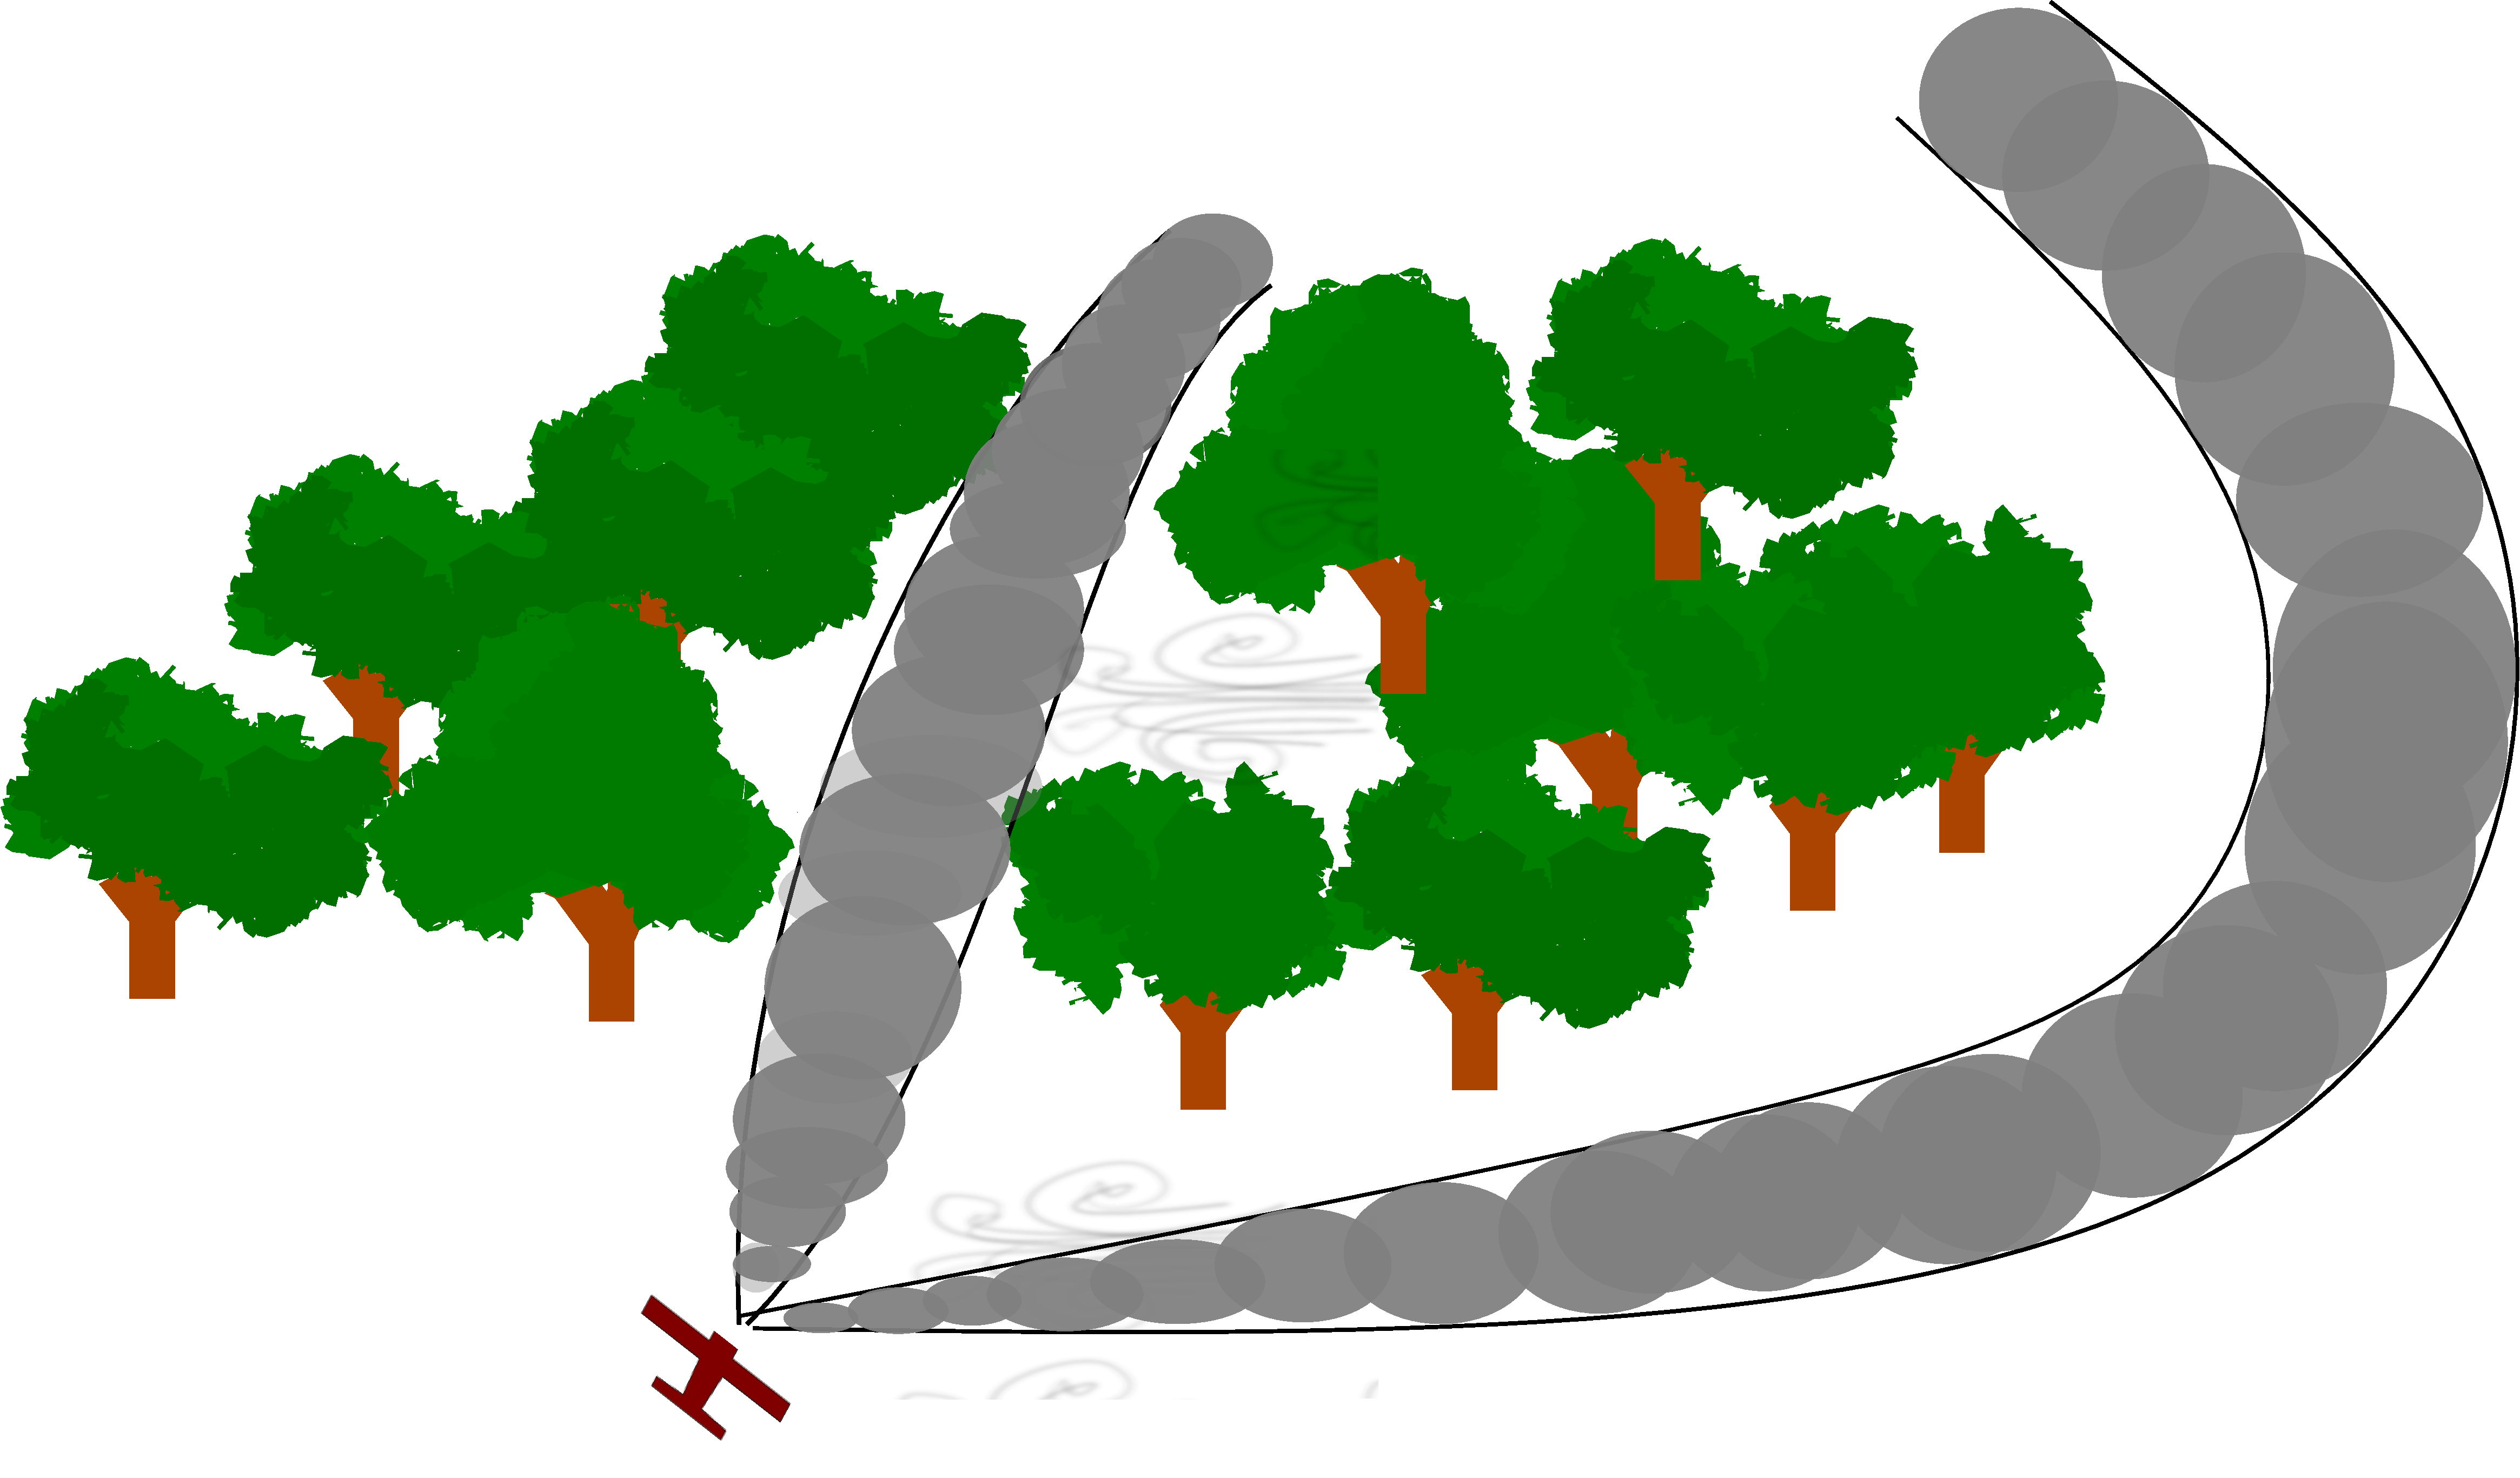
\includegraphics[scale=0.1]{figures/experiments/aggressive-maneuver}
  \caption{A planner that is guaranteed to not collide might as well go straight
    through the opening in the forest, instead of the long way around an
    obstacle.}
  \label{fig:aggressive-maneuver}
\end{figure}

\begin{figure}
  \centering 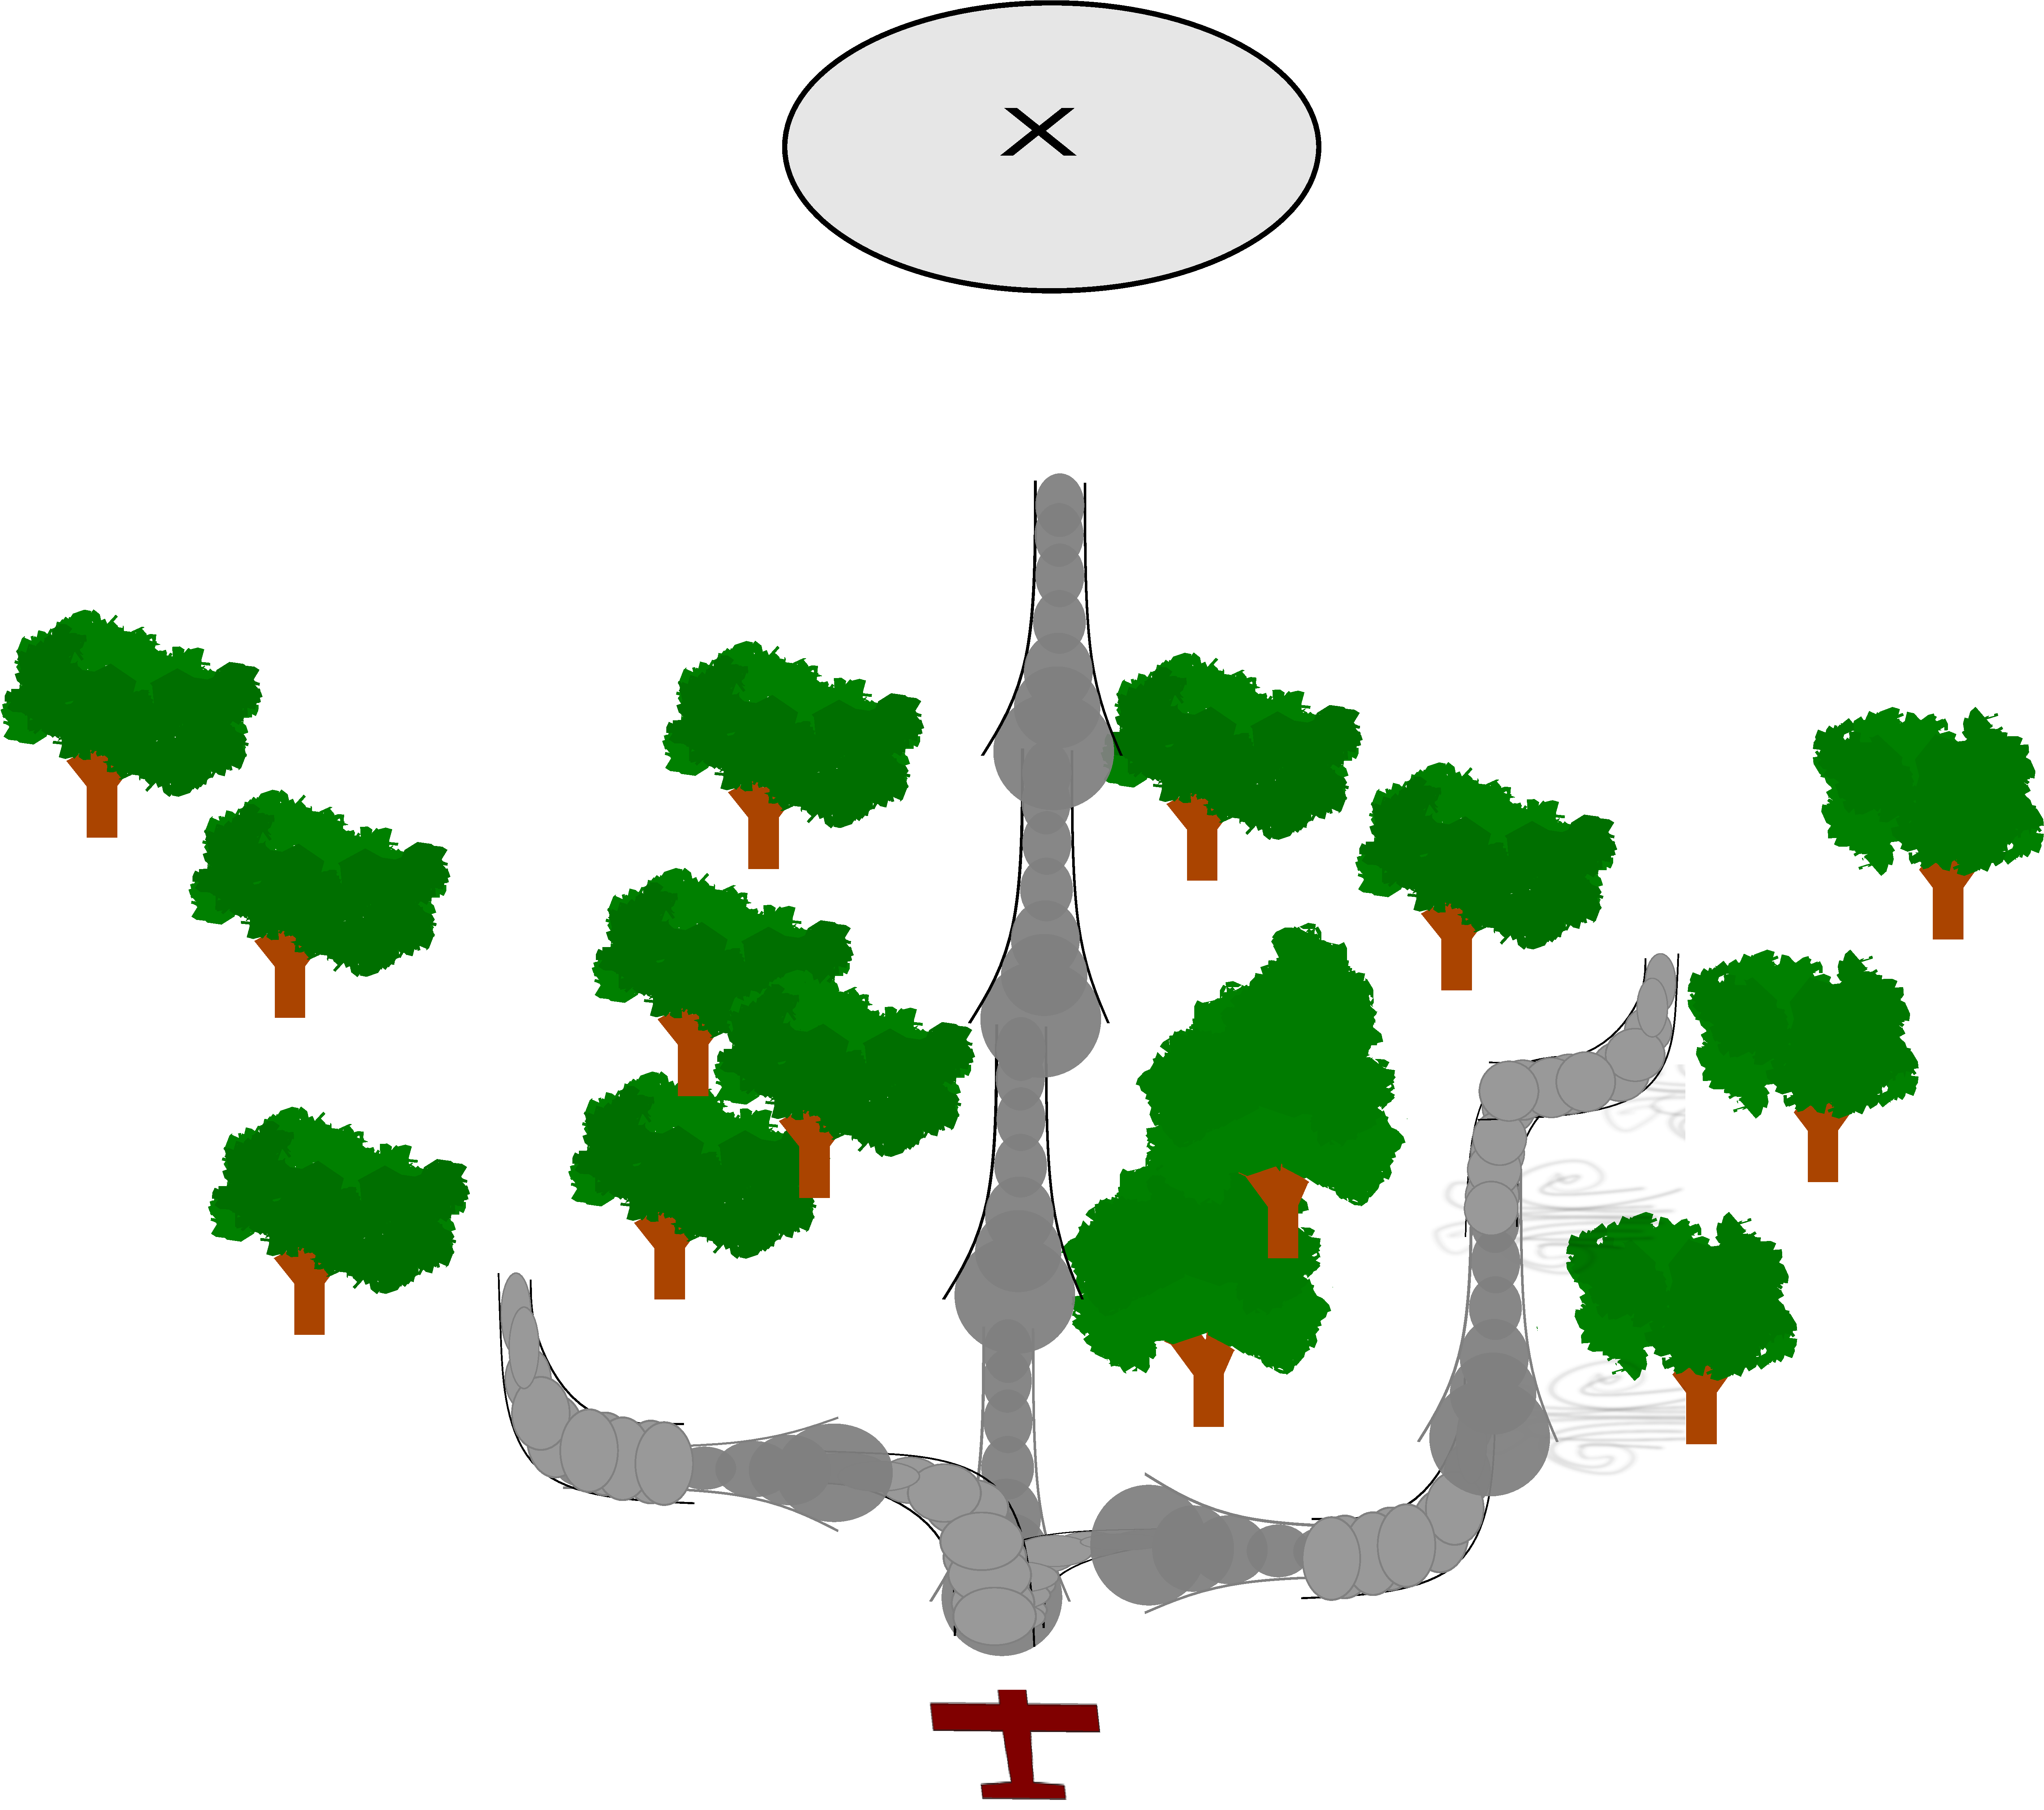
\includegraphics[scale=.1]{figures/experiments/experiment-airplane-strip}
  \caption{A cartoon of the experiment setup, showing how the \rrtfunnel{}
    algorithm builds a tree of funnels to find a safe path through the strip of
    forest.}
  \label{fig:experiments-airplane-strip}
\end{figure}

\begin{figure}
  \centering
  \missingfigure{experiment cartoon}
  \caption{The strip of forest that the airplane has to traverse safely in order
  for the planner to show that it handles uncertainty.}
\label{fig:experiment-cartoon}
\end{figure} 



\section{Outline}

The planning algorithm in this thesis is based on two 

This dissertation draws heavily on the earlier work and writing in the follow-
ing papers, written jointly with several collaborators:

\cite{majumdarFunnelLibrariesRealtime2017}

The rest of the thesis is organised as follows:
\begin{description}
    \item[\cref{chp:survey-of-papers}]
      provides a survey of current motion planning research focused on handling
      uncertainty in the environment, the system state and the surrounding
      environment, as well as some more in depth on the funnel theory employed
      in this thesis.
    
    \item[\cref{chp:preliminaries}]
      provides some introductory theory, first to motion planning as a general
      topic, then introduces the funnel generation theory through \ac{SOS}
      programming, and then develops the basic theory needed for understanding
      the inner workings of the \ac{RRT} algorithm.
    
    \item[\cref{chp:method}]
      develops the \rrtfunnel{} algorithm through two parts. Firstly it develops
      robust motion primtives through the \ac{SOS} programming framework. Then
      it develops the needed heuristics and sampling distribution for the
      \ac{RRT} motion planner and then incorporates the funnels from the first
      part as the extension operators to the tree that the algorithm builds
      through the configuration space.
    
    \item[\cref{chp:experiments}]
      contains the description of how to create and setup the experiment
      environment and the benchmark planner that is used in comparing the
      performance of the \rrtfunnel{} algorithm. The results follow right after.
    
    \item[\cref{chp:discussion}]
      gives a discussion of the results and a pointer to further work on the problem.

    \item[\cref{sec:first-app}]
      gives a basic introduction to the theory of \ac{SOS} verification of
      dynamical systems.

    \item[\cref{AppendixB}]
      contains some code examples from code. The rest of which can be found in \cite{my-code}.
\end{description}



